\subsection{以向量读取缓解共享指令队列压力}

共享内核的累加循环每步执行 \code{As[ty][k]} 与 \code{Bs[k][tx]} 两次共享读取，再完成一次乘加。对固定线程，连续四个 $k$ 对应的 $A$ 数据位于同一行相邻位置；相应的 $B$ 数据沿列分布，相邻地址间隔 $T$ 个元素。因此，可以把每线程连续的四个 $A$ 元素读成一个向量，$B$ 仍保留四次标量读取。

为了明确数据布局和对齐条件，可将 $A$ 的共享子块表示为自然 $16$ 字节对齐的 \code{float4} 数组。令 \code{As4[y][g]} 的四个分量依次保存原来的 $A$ 子块元素 $A^s_{y,4g},\ldots,A^s_{y,4g+3}$，并要求 $T$ 为正的 $4$ 的倍数。加载阶段使用对应的全局标量地址填入这些分量，在全部线程完成块内同步后，再执行代码\ref{l14:lst:vector-consume}所示的累加函数。该函数只表达消费端的向量读取机制，外层分块加载、边界补零及覆盖前同步仍按共享内核的规则处理。

\noindent\begin{minipage}{\linewidth}
\begin{lstlisting}[caption={对自然对齐的共享四元组进行向量读取},label={l14:lst:vector-consume}]
template<int T>
__device__ float accumulate_vector_tile(
    const float4 (&As4)[T][T / 4],
    const float (&Bs)[T][T],
    int ty, int tx, float sum) {
  static_assert(T > 0 && T % 4 == 0,
                "T must be a positive multiple of four");
  #pragma unroll
  for (int g = 0; g < T / 4; ++g) {
    float4 a = As4[ty][g];
    int k = 4 * g;
    sum += a.x * Bs[k + 0][tx];
    sum += a.y * Bs[k + 1][tx];
    sum += a.z * Bs[k + 2][tx];
    sum += a.w * Bs[k + 3][tx];
  }
  return sum;
}
\end{lstlisting}
\end{minipage}

这个表示让向量对象的类型和对齐条件明确，避免把任意未对齐地址直接解释成宽向量。每个线程仍需要相同的输入数值，并按相同的 $k$ 顺序累加；改变的是这些值进入寄存器时使用的读取指令宽度。是否最终生成一条宽共享加载，仍由编译结果决定，需要检查机器指令。

\begin{figure}[htbp]
\centering
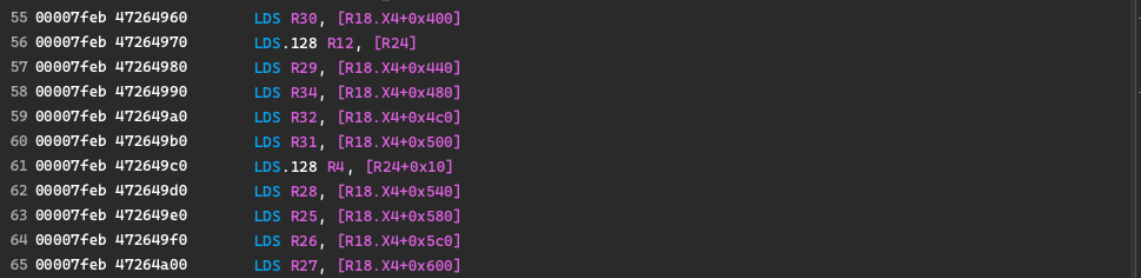
\includegraphics[width=0.92\textwidth]{vector_sass_detail.png}
\caption{共享向量读取对应的机器指令片段。宽指令 \code{LDS.128} 与保留的标量 \code{LDS} 同时存在，对应向量化的连续读取和其他标量读取。}
\label{l14:fig:vector-sass}
\end{figure}

以连续四次乘加为一个计数单位，原实现需要四次 $A$ 标量读取与四次 $B$ 标量读取，共 $8$ 次共享加载；向量化后需要一次 $A$ 宽读取与四次 $B$ 标量读取，共 $5$ 次。因此，理想共享加载请求的下降比例为
\begin{equation}
 r_{\mathrm{load}}=\frac{8-5}{8}=37.5\%.
 \label{l14:eq:vector-reduction}
\end{equation}
单看 $A$ 的读取指令，数量减少到四分之一；把 $A$、$B$ 都计入，整体减少到八分之五。四次乘加本身保持不变，所需标量数据量也保持不变。\code{LDS.128} 中的 $128$ 位是每线程的读取宽度，不能与一轮共享服务的 $128$ 字节混用。

\subsection{由指标变化验证优化机制}

表\ref{l14:tab:vector-case}给出原共享内核和改进版的比较。共享加载从约 $211.76$ 百万降到 $132.35$ 百万，下降 $37.50\%$，与式\eqref{l14:eq:vector-reduction}一致。共享存储请求保持约 $13.24$ 百万，因此计入写入后的共享总指令下降比例较小，为约 $35.29\%$。

\begin{table}[htbp]
\centering\small
\caption{共享读取向量化前后的报告变化}
\label{l14:tab:vector-case}
\begin{tabularx}{\textwidth}{@{}Yrrr@{}}
\toprule
指标 & 共享分块 & 共享改进版 & 相对变化\\
\midrule
共享加载请求（百万） & $211.76$ & $132.35$ & $-37.50\%$\\
共享存储请求（百万） & $13.24$ & $13.24$ & $0\%$\\
共享总指令（百万） & $225.00$ & $145.59$ & $-35.29\%$\\
全局存储空间指令（百万） & $13.29$ & $13.29$ & $0\%$\\
设备内存读取量（GB） & $1.24$ & $1.23$ & 约 $-1.34\%$\\
\bottomrule
\end{tabularx}
\end{table}

表中的数据量经过舍入，相对变化可能由更高精度的报告计数计算。例如 $1.24$ GB 与 $1.23$ GB 的显示值不足以重现 $-1.34\%$ 的报告变化，应将其解释为小幅下降。

全局加载请求与全局指令基本保持不变，设备内存读取量也只有小幅波动，这与局部修改共享读取方式的范围相符。图\ref{l14:fig:vector-evidence}的指令组合显示共享加载显著减少，浮点乘加数量保持不变；总执行指令下降约 $15.32\%$。因此，这次改进的主要证据是减少共享加载指令与队列压力，而非显著改变设备内存流量。

\begin{figure}[htbp]
\centering
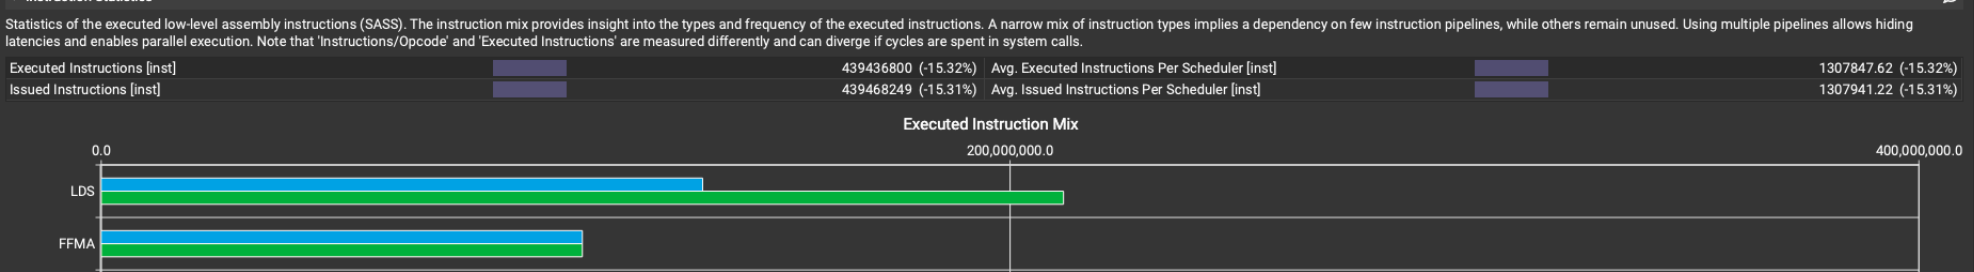
\includegraphics[width=\textwidth]{instruction_comparison.png}
\caption{共享改进版与原共享版本的指令组合比较。上方共享加载条带缩短，下方单精度乘加条带基本重合，说明算术工作保留而读取指令减少。}
\label{l14:fig:vector-evidence}
\end{figure}

线程束状态比较也与这个机制相符。图\ref{l14:fig:stall-comparison}中，存储输入输出节流的平均周期约从 $24.4$ 降到 $16.0$；部分其他等待没有同步下降，长记分板等待还略有增加。这并不破坏当前解释，因为优化针对的是主要共享指令压力，总执行指令和主要等待已经减少。

\begin{figure}[H]
\centering
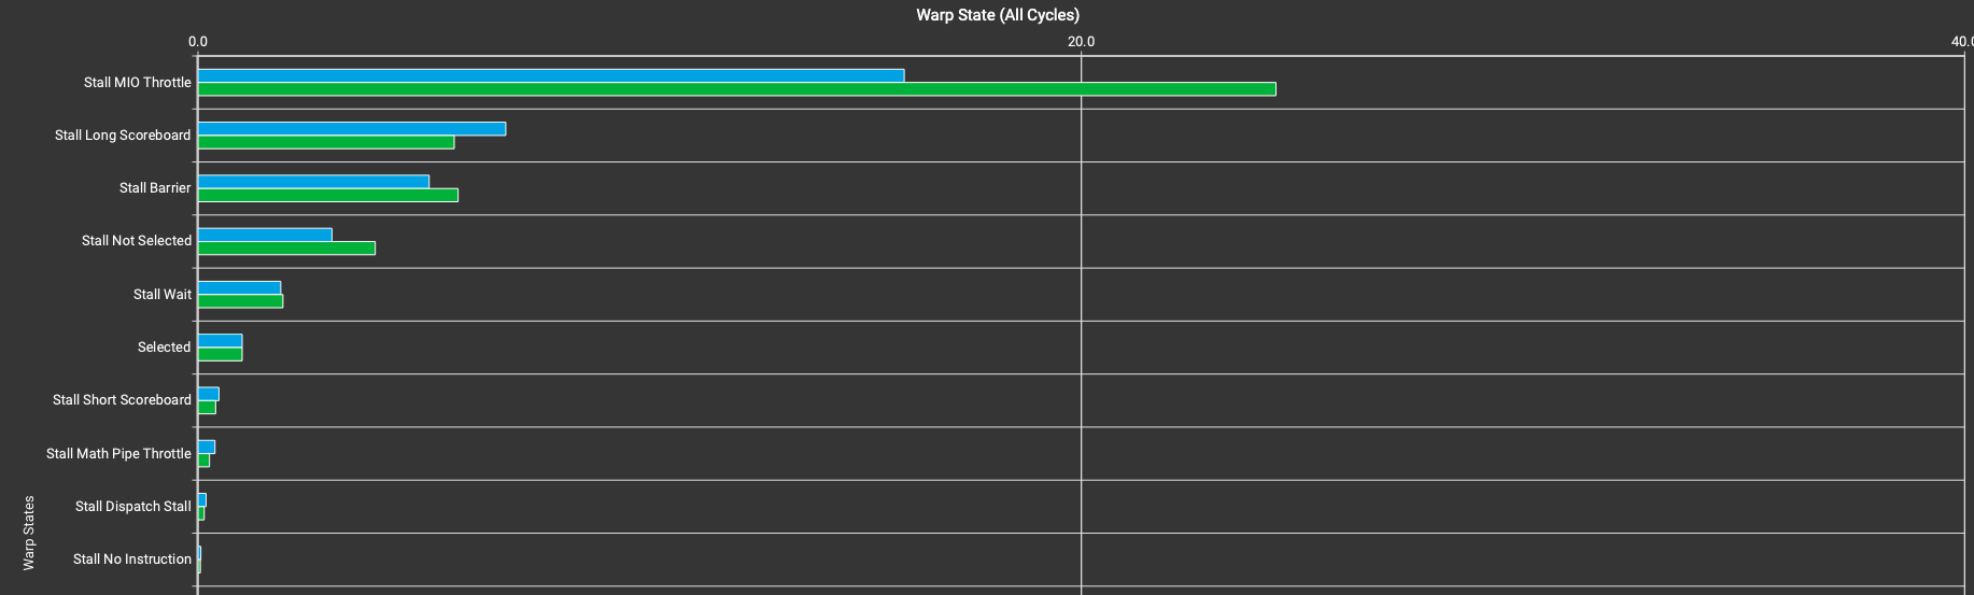
\includegraphics[width=0.9\textwidth]{stall_comparison.png}
\caption{共享改进版与原共享版本的线程束状态比较。蓝色对应改进版，绿色对应原共享版本；主要变化是存储输入输出节流降低，其他等待不必按相同比例变化。}
\label{l14:fig:stall-comparison}
\end{figure}

最后回到正常 CUDA 事件计时。A40 上耗时从 $3.34$ 毫秒降至 $2.29$ 毫秒，相对原共享版本达到约 $1.46$ 倍加速；L40S 上从 $1.92$ 降至 $1.31$ 毫秒，约为 $1.47$ 倍；B200 上从 $1.35$ 降至 $1.07$ 毫秒，约为 $1.26$ 倍。总时间没有按共享加载请求的比例直接下降，因为全局读取、共享写入、乘加、同步及其他指令仍然存在，减少某一类请求也不等于消除了所有等待。

进一步优化时，多余扇区提示检查线程映射与对齐，片上加载繁忙提示考虑寄存器复用，寄存器用量压低驻留数量则提示调整粗化程度或分块形状。修改后应核对相关计数器、数值结果及同条件计时。

\begin{keybox}[title={性能诊断的关键关系}]
诊断应同时联系工作量、指令数、各层流量、驻留资源与发射状态，并用总时间判断修改的收益。
\end{keybox}
